
\documentclass[11pt]{article}
\usepackage{natbib}
\usepackage{common}

\title{HW2: Language Modeling}
\author{Alex Lin \\ alexanderlin01@college.harvard.edu \and Melissa Yu \\ melissayu@college.harvard.edu }
\begin{document}

\maketitle{}
\section{Introduction}

Language modeling is a very interesting problem that has experienced much development over the past few years.  The central idea is to build a statistical model that can accurately estimate the distribution of natural language.  For this problem set, we examined the issue of trying to predict the 20 most likely words for continuing a pre-specified sentence.  We examined three main models for this problem: (1) a basic trigram model, (2) a neural network language model (NNLM), and (3) a long short term memory recurrent network model (LSTM).  We tuned this models to try to optimize \emph{perplexity}, our metric of choice that measures how well a probability distribution predicts a sample.

\section{Problem Description}

Let $\mathcal{V}$ be the vocabulary.  We assume words are represented as one-hot encoded vectors of size $\lvert \mathcal{V} \rvert \times 1$.  Given a sequence of words encoded as one-hot vectors $\boldx_1, \boldx_2, \ldots, \boldx_N$, the objective is to accurately predict the distribution of $\boldx_{n + 1} \vert \boldx_1, \ldots, \boldx_{n}$ for $n = 1, 2, \ldots, N$.  Let $q$ be our model's predictive distribution.  The objective is to adjust the model's parameters to minimize the \emph{average loss}, as defined by
\begin{align*}
L = \frac{1}{N} \sum_{n=1}^N \left(\ln q(\boldx_{n + 1} \vert \boldx_1, \ldots, \boldx_{n}) \right) \cdot x_{n+1} 
\end{align*}
where $\cdot$ denotes the inner dot product.  The standard metric used for evaluation is called \emph{perplexity}, as defined by
\begin{align*}
P = \exp L
\end{align*}

\section{Model and Algorithms}

We trained the three different models specified in the instructions.  These included (1) a basic trigram model, (2) a neural network language model (NNLM), and (3) a long short term memory recurrent network model (LSTM).

\subsection{Trigram Model}

\subsection{Neural Network Language Model}


\subsection{Long Short-Term Memory Recurrent Neural Network Model}
The Long Short-Term Memory Recurrent Neural Network Model (LSTM) was proposed as a way to cleanly integrate long-term memory into a recurrent neural network.  Traditionally, regular recurrent neural nets have suffered from an inability to propagate information from past iterations of training, because they get inundated with more recent information.  The LSTM has four interacting layers, as depicted below.  This helps with deciding what information to propagate or forget from earlier in sentences.  The key idea is that there is a cell state $\boldC_t$ that may or may not be modified significantly by operations applied to the hidden state propagated hidden state $\boldh_t$ and the current word $\boldx_t$. 

\begin{figure}[H]
\begin{center}
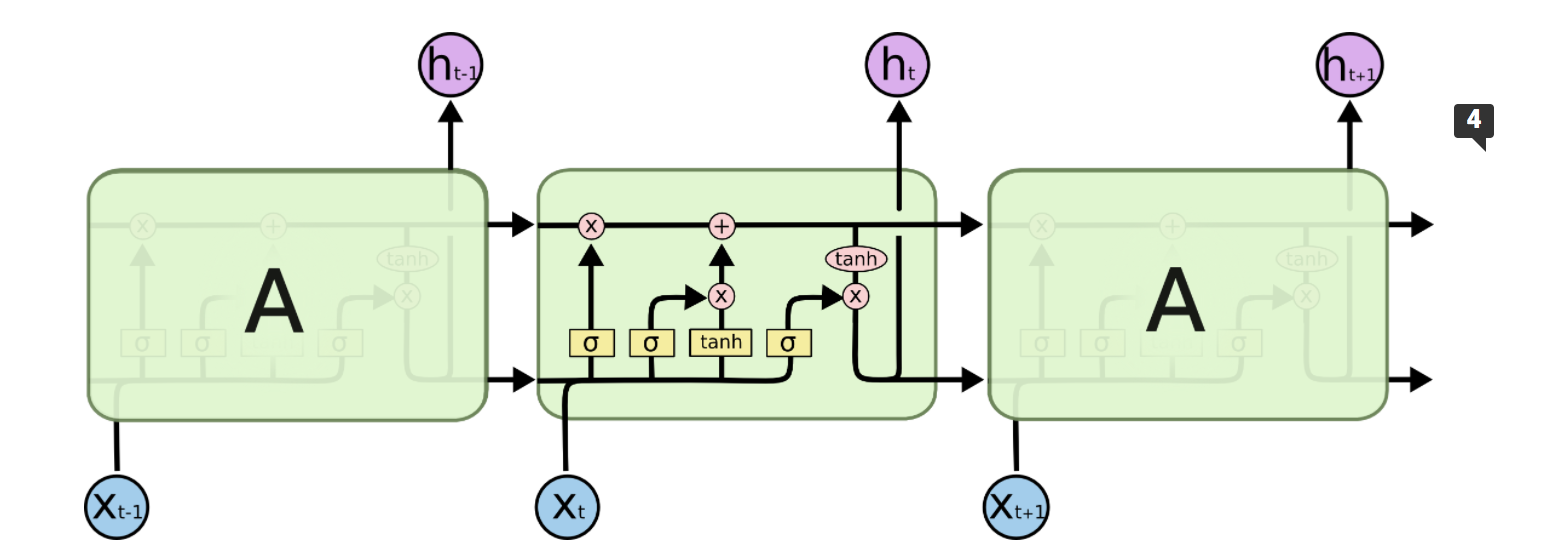
\includegraphics[scale=0.5]{lstm}
\caption{An unrolled diagram of a single-layer LSTM.}
\end{center} 
\end{figure}

\noindent
The mathematical layering of a single-layer LSTM follows:
\begin{align*}
\boldf_t &= \sigma(\boldW_f \cdot [\boldh_{t-1}, \boldx_t] + b_f) \\
\boldi_t &= \sigma(\boldW_i \cdot [\boldh_{t-1}, \boldx_t] + b_i) \\
\tilde{\boldC}_t &= \tanh(\boldW_C \cdot [\boldh_{t-1}, \boldx_t]  + b_C) \\
\boldC_t &= \boldf_t * \boldC_{t-1} + \boldi_t * \tilde{\boldC} \\
\boldo_t &= \sigma(\boldW_o \cdot [\boldh_{t-1}, \boldx_t]  + b_o) \\
\boldh_t &= \boldo_t * \tanh(\boldC_t)
\end{align*}
where $*$ denotes the element-wise multiplication operator. 

For the construction of the overall model to predict the distribution over the next word $\boldx_{t+1}$, we follow the architecture as described by Zaremba et. al in their "large regularized LSTM".  We first encode each word as an embedding $\boldx_t$ of size $d \times 1$.  Then, we pass $\boldx_t$ through a 2-layer LSTM with $l =1500$ hidden units to get an output $\boldo_t$.  For regularization, we then apply dropout with a rate of 0.65 to $\boldo_t$.  Next, we apply a linear transformation to $\boldo_t$ and pass the result through a softmax function to obtain a probability distribution $\boldq_t$ over the next word:
\begin{align*}
\boldq_t = \text{softmax} (W \boldo_t + b)
\end{align*} 
where $W$ is a $\lvert \mathcal{V} \rvert \times l$ matrix and $b$ is a $\lvert \mathcal{V} \rvert \times 1$ vector.  This $\boldq_t$ is then used to calculate the average loss.  We adjust weights to reduce the average loss using different optimizers such as stochastic gradient descent and Adam.  For final comparisons between models of this type, we report perplexity on the test set.           


\section{Experiments}

We performed several experiments to tune the hyper-parameters of our models.  In general, the LSTM seemed to perform the best.  In-depth explanations of our tuning procedure and associated results can be found in this section.  Note that all perplexities are test set perplexities. 

\begin{table}[H]
\centering
\begin{tabular}{llr}
 \toprule
 Model &  & Acc. \\
 \midrule
 \textsc{Trigram Model} & &  \\
 \textsc{Neural Network Language Model} & &  \\
 \textsc{Long Short-Term Memory RNN} & & 139.98 \\
 \bottomrule 
\end{tabular}
\caption{\label{tab:results} Language perplexities of our models.}
\end{table}

\subsection{Trigram Model} 

\subsection{Neural Network Language Model}

\subsection{Long Short-Term Memory RNN}
One item we varied in the LSTM RNN was the number of hidden states for the LSTM.  Specifically, we looked at differences between the "medium-size" LSTM (650 states) and the "large-size" LSTM (1500 states) proposed by Zaremba et. al.  We found that the large-size LSTM took longer to train, but obtained a significantly lower perplexity.  However, the difference is large enough, so we decided to stick with large LSTM.  Here are our best results on both models.

\begin{center}
	\begin{tabular}{ c | c c c c c}
		 & Medium LSTM & Large LSTM  \\
		\hline
		Test Set Perplexity & 160.12 & 139.98 
	\end{tabular}
\end{center} 

The second variable that we took into account was the optimization method.  We looked at both SGD and Adam.  We also varied the \emph{starting} learning rate (STR) for these two methods.  During training, we followed the results in the paper and decreased the learning rate by a factor of 1.2 for each iteration.  Here are our best result under various settings.     

\begin{center}
	\begin{tabular}{ c | c c c c c}
		 & SGD (STR = 1) & SGD (STR = 0.1) & SGD (STR = 0.01)  \\
		\hline
		Test Set Perplexity & 203.27 & 156.35 & 183.24 
	\end{tabular}
\end{center} 

\begin{center}
	\begin{tabular}{ c | c c c c c}
		 & Adam (STR = 0.01) & Adam (STR = 0.001)  \\
		\hline
		Test Set Perplexity & 152.12 & 139.98 
	\end{tabular}
\end{center} 
From this, we chose to use the Adam optimizer with a starting learning rate of $10^{-3}$.  

The last variable we looked at was varying the word embedding dimension $d$.  Surprisingly, this had quite a significant effect on the efficacy of the LSTM RNN.  Here are our best results. 

\begin{center}
	\begin{tabular}{ c | c c c c c}
		 & $d = 100$ & $d = 300$ & $d = 500$ &  $d = 1000$  \\
		\hline
		Test Set Perplexity & 189.21 & 151.20 & 143.44  & 139.98 
	\end{tabular}
\end{center}    

Thus, we decide to use an embedding size of 1000.

\section{Conclusion}



\bibliography{writeup}
\nocite{*}
\bibliographystyle{apalike}

\end{document}
